\subsubsection{Deployment Patterns} 
\label{cloud-measure-feature}

In this section, we use the DNS records from our \alexadata dataset and a 
variety of
heuristics to detect and quantify usage of the deployment patterns
outlined in \figref{fig:ec2_models}. Specifically, we estimate the use
of virtual machines (VMs), platform-as-a-service (PaaS) environments,
load balancers, content-distri\-bu\-tion networks (CDNs), and domain name
servers within the \frontends of web services hosted in both EC2 and
Azure. In general, we discuss EC2 and Azure separately because of
differences in the cloud architectures.

\tightparagraph{VM \frontend in EC2} 
Each VM instance in an IaaS cloud combines a set of virtual resources (CPU
core(s), memory, local storage, and network bandwidth) whose capacity depends
on the instance type.  In EC2 each instance is assigned an internal IP
address within a region-specific private network; EC2 tenants may optionally
assign a public (i.e., Internet-routable) IP address to a VM.  

We identify usage of VMs as directly-reachable web service 
\frontends---i.e., deployment pattern {\em P1} (\figref{fig:ec2_vm})---by examining
if the DNS query for an EC2-using subdomain directly returns an IP
address (instead of a CNAME), which we then associate with a VM
instance.
We find that 505,578 (72\%) EC2-using subdomains leverage \frontend VMs.
\figref{fig:Alexa_ec2_non_elbs_CDF} shows a CDF of the number of \frontend VM
instances used by each EC2-using subdomain; this CDF only includes subdomains
which use \frontend VMs. We observe that about half of such subdomains use 2
\frontend VMs and 15\% use 3 or more \frontend VMs. 

\begin{figure}[t]
\centering

\begin{subfigure}[b]{0.4\textwidth}
    \caption{Virtual machine instances}
    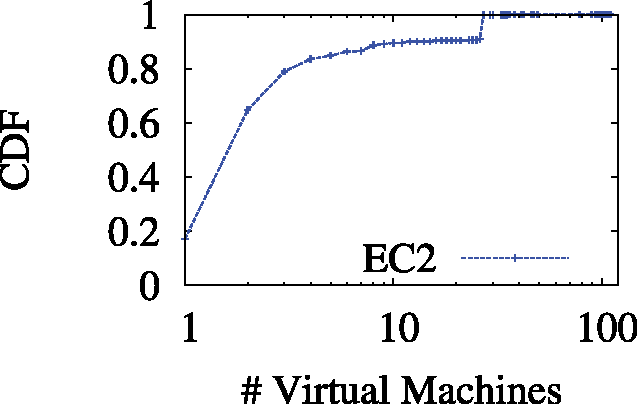
\includegraphics[width=\textwidth]{figures/cloudmeasure/imag_sec3/subdomain_vm_cdf.pdf}
    \label{fig:Alexa_ec2_non_elbs_CDF}
\end{subfigure}
\begin{subfigure}[b]{0.4\textwidth}
    \caption{Physical ELB instances}
    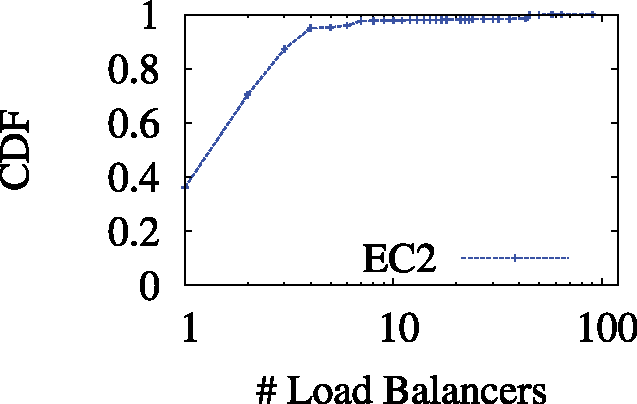
\includegraphics[width=\textwidth]{figures/cloudmeasure/imag_sec3/subdomain_elb_cdf.pdf}
    \label{fig:Alexa_ec2_elbs_CDF}
\end{subfigure}

\caption{CDFs for the \# of feature instances per subdomain (only includes
        subdomains which use the feature).}
\label{fig:Alexa_feature_CDF}
\end{figure}

\begin{figure}
    \centering
    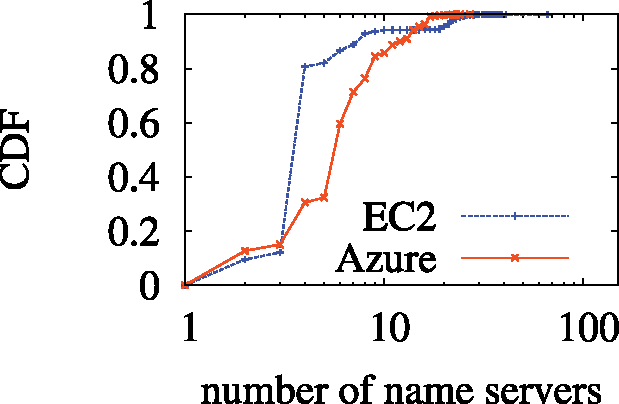
\includegraphics[width=0.50\columnwidth]{figures/cloudmeasure/imag_sec3/subdomain_ns_cdf.pdf}
    \caption{CDF of the \# of DNS servers used per subdomain.}
    \label{fig:Alexa_ns_subdomain_cdf}
\end{figure}



Aggregating by domain, we find that 52\% of EC2-using domains have at least
one subdomain which uses at least one \frontend VM. If we sum the number of
\frontend VMs used across all subdomains of a given domain, we find that 10\%
of domains which use \frontend VMs in EC2 use 3 or more \frontend VMs in
total. % (omitted for brevity).

\tightparagraph{PaaS \frontend in EC2} 
PaaS systems offer a hosted environment for deploying web applications, 
avoiding the need for tenants to manage low-level system details. PaaS
systems are frequently built atop existing IaaS infrastructure: e.g.,
Amazon's Elastic Beanstalk and Heroku
both run atop EC2. A Beanstalk environment always includes an Amazon Elastic
Load Balancer (ELB) instance (discussed in more detail below), reflecting
deployment pattern  {\em P2} (\figref{fig:ec2_elb}, replace
VMs with PaaS nodes). A Heroku environment may or may not include an ELB,
reflecting usage of deployment patterns {\em P2} or {\em P3}
(\figref{fig:ec2_models}), respectively.


We say that a subdomain uses Beanstalk or Heroku if the subdomain's DNS
record has a CNAME 
that ({\em i}) includes `elasticbeanstalk' or any of `heroku.com',
`herokuapp', `herokucom', and `herokussl' and ({\em ii}) resolves to
an IP in EC2's public IP address range. In the case of Heroku without ELB,
the IPs to which the CNAME resolves represent PaaS nodes; we associate these
IPs with the subdomain whose DNS record contains the corresponding CNAME.



 
A total of 201,666 (28\%) EC2-using subdomains in our \alexadata
dataset contain
a CNAME in their DNS record. Applying the above filters for PaaS, we
find that 60,273 (8\%) EC2-using subdomains use a \frontend PaaS
environment in EC2. Of these, over 97\% (59,991) are using Heroku;
only 3\% use Elastic Beanstalk. Amazon always includes an ELB in a  
Beanstalk environment, but Heroku only sometimes leverages ELBs---only 3\% of
subdomains (1,850) which use Heroku also use ELB.
We therefore conclude that,
in the case of EC2, PaaS systems are predominantly used according to
deployment pattern {\em P3} (\figref{fig:ec2_paas}).

We now focus on the 58,141 (59,991 - 1,850) subdomains that use
Heroku without ELB. We find that these are associated with just
94 unique IPs. Although we have no insight into the number of worker
instances used by Heroku, this shows that Heroku is multiplexing PaaS
functionality among a relatively large number of subdomains: in
particular, we find that about one-third of subdomains using
Heroku share the CNAME `proxy.heroku.com'.
 
\tightparagraph{Load balancer \frontend in EC2} 
Load balancers divide traffic among a set of ``worker'' VMs or PaaS nodes, as
reflected in deployment pattern {\em P2} (\figref{fig:ec2_elb}).
Amazon Elastic Load Balancers (ELBs) are Amazon-managed
HTTP proxies. An EC2 tenant requests an ELB in a specific region and
subsequently associates VM instances, in one or more zones, with this ELB.
The ELB automatically round-robins requests among zones and among the VMs in
each zone.  In fact, traffic is routed to zone-specific ELB proxies by
rotating the order of ELB proxy IPs in DNS replies. ELB can also
be used with PaaS, as discussed above.  

When a subdomain uses an ELB, the subdomain's DNS record contains a
CNAME ending in `elb.amazonaws.com'; the
CNAMEs resolve to IP addresses for one or more ELB proxies.  We identify
ELB-using subdomains in our \alexadata dataset based on the presence of such 
CNAMEs; we refer to each distinct CNAME as a ``logical ELB
instance''. We also associate with the subdomain the IPs of the specific ELB
proxies to which the CNAME resolves; we refer to these as ``physical ELB
instances''.

We find that 27,154 (4\%) EC2-using subdomains use ELB as their \frontend.
Of the subdomains that use ELB, 280 (1\%) use it in the context of Elastic
Beanstalk and 1,850 (6.8\%) use it with Heroku.  Aggregating by domain, we
find that 9,851 (26\%) EC2-using domains use \frontend ELB(s).

Across all ELB-using subdomains, we observe 15,703 physical ELB instances
(i.e., distinct IPs associated with ELB CNAMEs).
Hence, while each subdomain has its own logical ELB(s), the
physical ELB proxies that perform the actual load balancing appear to
be shared across multiple, even unrelated, subdomains. In particular, we 
analyzed the number of subdomains per
physical ELB and found that $\approx$4\% of the physical ELB instances are
shared by 10 or more subdomains.% (details omitted for brevity).



\figref{fig:Alexa_ec2_elbs_CDF} shows a CDF of the number of physical ELB
instances associated with each subdomain; this CDF only includes subdomains
which use ELB. We observe that about 95\% of ELB-using subdomains are
associated with 5 or fewer physical ELB instances. A few ELB-using 
subdomains (e.g., dl.outbrain.com and m.netflix.com) use many
physical ELB instances: 58 and 90, respectively.

\iffalse
\tightparagraph{Front ends in Azure}
Azure's architecture differs from EC2 insofar as clients cannot distinguish
whether a web service uses a VM, PaaS, or load balancer
\frontend. In Azure, VMs and PaaS environments are both encompassed within
logical ``Cloud Services'' (CS). An individual CS may contain ({\em i}) a
single VM, ({\em ii}) a collection of related VMs, or ({\em iii}) a PaaS
environment.  Each CS is assigned a unique DNS name ending with
`cloudapp.net' and a corresponding public IP address.  
Traffic sent to this public IP goes through a transparent
proxy---which performs NAT and, optionally, load balancing---before directing
traffic to a VM or PaaS node.  Thus, a CS may reflect deployment patterns
{\em P1}, {\em P2} (with VMs or PaaS nodes), or {\em P3} (\figref{fig:ec2_models}), all of which appear
the same from a client perspective.

We examine the DNS records for Azure-using subdomains in the
\alexadata dataset to identify subdomains which use a CS (i.e., VM, PaaS, or
load balancer) \frontend.  If the DNS query for
an Azure-using subdomain either directly returns an IP address or
returns a CNAME ending in `cloudapp.net', then we say the subdomain
uses a CS \frontend. We associate the directly returned IP or the
CNAME, and its corresponding IP, with a CS instance.

A total of 1,153 (17\%) Azure-using subdomains directly resolve to an IP
address and 5,404 (82\%) Azure-using subdomains contain a CNAME in their DNS
record.  Applying the above filters for CS, we find that 4,581 (70\%)
Azure-using subdomains use a CS \frontend.  Aggregating by domain, we find that 57\% of Azure-using domains
have at least one subdomain which uses a CS \frontend. 

Azure also offers a unique feature (which has no parallel in EC2) for load
balancing across \frontends: Azure Traffic Manager
(TM) uses DNS to direct traffic to different CSs, which
may be spread across multiple regions.  TM can, based on a tenant's
preference, do performance-based load balancing (finding the CS closest to
the client), failover load balancing (picking the next active CS), or simple
round-robin load balancing.  When a subdomain uses TM, its DNS record
contains a CNAME ending in `trafficmanager.net', similar to ELB.  However, TM
performs all load balancing using DNS---unlike ELB which uses a combination
of DNS and physical proxies---so TM CNAMEs resolve directly to a CNAME for a
specific CS (e.g., `abc.cloudapp.net').  We find that only 100 (2\%)
Azure-using subdomains (corresponding to 52 domains) use TM. 


The aforementioned CNAME-based filters for ELB, Beanstalk, Heroku, CS,
and TM were not applicable to 116,323 (16\%) EC2-using
subdomains, and 1,938 (30\%) Azure-using subdomains. We are
investigating techniques to understand the deployment patterns
underlying these subdomains.
\fi

\tightparagraph{Content distribution networks}  We now focus on the use
of CDNs, which we illustrated in deployment pattern {\em P4}
(\figref{fig:ec2_cdn}). Note that CDNs can be employed alongside any of the
other three deployment patterns.

Both Microsoft and Amazon run their own CDNs, which we focus on
studying. Amazon's CloudFront CDN uses a
different public IP address range than the rest of EC2. Hence, we
determine if a subdomain uses CloudFront by observing if its DNS
records contain one or more IPs in CloudFront's IP range.
Azure's CDN uses the same IP address ranges
as other parts of Azure, so we detect whether a subdomain
uses the Azure CDN based on whether a subdomain's DNS records contain
CNAMEs with `msecnd.net'.

We find 7,622 subdomains (corresponding to 5,988 domains) use CloudFront and
68 subdomains (corresponding to 54 domains) use Azure's CDN. 
Despite the much smaller number of domains using Azure's CDN, there is
still a significant volume of traffic associated with msecnd.net
in our \capturedata dataset (\tabref{tab:topdomains}). Azure's CDN is clearly
being used within some Microsoft properties, perhaps to host embedded
content or cookies.


\tightparagraph{Domain name servers} The first step in accessing a
cloud-resident service is to resolve its name
(\figref{fig:ec2_models}). In what follows, we examine cloud-resident
subdomain's use of DNS, focusing on the extent to which they rely on
cloud providers for DNS services as well.

%  versus employing DNS hosted
% outside the cloud. 

We identifed the ``location'' of a cloud-using subdomain's
authoritative name server(s) as follows: For each DNS record
associated with a given subdomain in our \alexadata dataset, we
extract all the domains specified in the NS records. We then performed
a DNS lookup on each of these domains from 50 globally-distributed
PlanetLab nodes. We flushed and reset the cache of the local resolver
between each DNS lookup, and we added the `norecurse' flag to each
DNS query to minimize the influence of caching. We compare the
resulting IP addresses to the public IP address ranges for EC2,
CloudFront, and Azure.

We observe a total of 23,111 name servers supporting the 713K
cloud-using subdomains in our \alexadata dataset. Many subdomains use
the same name servers, leading to a smaller set of name servers than
subdomains. \figref{fig:Alexa_ns_subdomain_cdf} shows a CDF for the
number of name servers used by each cloud-using subdomain; we observe
that nearly 80\% of subdomains use 3 to 10 name servers. We
categorize the name servers as follows: 2,062 were hosted in
CloudFront, which appears to host Amazon's route53 DNS service as many
of these name servers had `route53' in their domain name; 1,239 were running
inside EC2 VM instances; 22 were hosted inside Azure VM instances
or Azure CS; and 19,788 were
hosted outside any of EC2, CloudFront, or Azure; 


\begin{table}[tb]
\centering
\small
\setlength{\tabcolsep}{0.1cm}
\begin{tabular}{|c|c|r|r|r|} \hline
{\bf Cloud }&\bf{Feature} & {\bf \# Domains} & {\bf \# Subdomains } & {\bf
    \# Inst.} \\
\hline
\multirow{5}{*}{EC2}
& VM & 19.9K (52.5\%)  &  505.6K (71.5\%) & 28.3K \\ \cline{2-5}
%& ELB-BeanStalk & 9.7K (25.5\%) & 26.9K (3.8\%) & 15.3K\\\cline{2-5}
& ELB & 9.9K (25.9\%) & 27.1K (3.8\%) & 15.7K\\\cline{2-5}
& BeanStalk (w/ ELB) & 188 (0.5\%) & 280 ($<0.01$\%) & 455  \\ \cline{2-5}
& Heroku (w/ ELB & 622 (1.6\%)  & 1.9K (0.3\%) &  2.4K\\ \cline{2-5}
& Heroku (no ELB) & 1.3K (3.5\%)  & 58.1K (8.2\%) &  94\\ \cline{2-5}
%& CloudFront CDN & 137 & n.a. \\ \cline{2-4}
%& Route53 DNS & 2,041  \\ 
\hline
\hline
\multirow{2}{*}{Azure}
%  & VM  & 455 (19.5\%) & 1.2K (17.6\%) & 720\\ \cline{2-5}
%  & CS+TM & 52 (2.2\%) & 100 (1.5\%) & 78\\ \cline{2-5}
%  & CS-TM & 825 (35.3\%) & 3.3K (50.8\%) & 790\\ \cline{2-5}
  & CS & 863 (37.0\%) & 4.5K (68.3\%) & 790\\ \cline{2-5}
  & TM & 52 (2.2\%) & 100 (1.5\%) & 78\\ \cline{2-5}
  %& msecnd CDN & ... & ...\\ 
\hline
\end{tabular}


%%%%%%%%%%%%%%%%%%%%%%%%%%%%%%%%%%%%%%%%%%%bkp%%%%%%%%%%%%%%%%%%%%%%
\iffalse
\begin{tabular}{|c|c|r|r|r|} \hline
{\bf Cloud }&\bf{Feature} & {\bf \# Domains} & {\bf \# Subdomains } & {\bf
    \# Instances} \\ 
\hline
\multirow{4}{*}{EC2}
& VM & 19,896 (52\%)  &  505,578 (72\%) & 28,258 \\ \cline{2-5}
& LB & 9,851 (26\%) & 27,154 (4\%) & 15,703\\\cline{2-5}
& PaaS & 1,929 (5\%) & 60,273 (8\%) & 2,979  \\ \cline{2-5}
& LB + PaaS & 809 (2\%)  & 2,130 (0.3\%) &  2,890\\ \cline{2-5}
%& CloudFront CDN & 137 & n.a. \\ \cline{2-4}
%& Route53 DNS & 2,041  \\ 
\hline
\hline
\multirow{4}{*}{Azure}  
  & VM  & 455 (19\%) & 1,153 (18\%) & 720\\ \cline{2-5}
  & LB & 52 (2\%) & 100 (2\%) & 78\\ \cline{2-5}
  & PaaS & 863 (37\%) & 3,428 (52\%) & 864\\ \cline{2-5}
  & LB + PaaS & 52 (2\%)  & 100 (2\%) & 78 \\ \cline{2-5}
  %& msecnd CDN & ... & ...\\ 
\hline
\end{tabular}
\fi


\caption{Summary of cloud feature usage.
}
\label{tab:features-used}
\end{table}

The above analyses are summarized in \tabref{tab:features-used} which
shows how many (sub)domains in our \alexadata dataset use each cloud
feature. We also show the number of instances (identified by IP
address) of that feature. 


\begin{table}[t]
\centering
\small

% \begin{tabular}{|c||c|c|c|c|c|c|c|c|c|c|c|} \hline
% Rank& domain & \# sub& \# ELB & sub/ELB & \#  PaaS & sub/PaaS & \# VM & sub/VM & CDN\\ \hline
% 9      & amazon.com &2 &27& 1.0& 3& 1.0 &-& -&N \\ \hline %1,3,u
% 13      & linkedin.com  & 3& 1& 1.0& 26& 1.0 &- &-& N\\ \hline %1,u
% 35      & pinterest.com         & 18 &0 &0 &0& 0& 40& 2.0 &N \\ \hline %u, 2
% 36      & fc2.com   &14 &68& 1.0& 0& 0& 32& 1.0  &N \\ \hline % 1,2,3
% 48     & imdb.com         & 2& 0& 0& 0& 0& - &- & Y \\ \hline % 3
% 59     & go.com      & 4 &32 &1.0& 18& 1.0 & - & - & N \\ \hline % n/a
% 75     & instagram.com        &6 &1 &1.0 &0& 0 &36 &1.9 &Y \\ \hline % 2, 3
% 86     & imgur.com       & 1 &0 &0& 0& 0 & - & - & N \\ \hline % 1, 3
% 92     & netflix.com    & 15 &104& 4.3& 0& 0& - & - &  N\\ \hline % 4
% 119     & dropbox.com         &9 &0& 0& 0 &0 &3 &1.7 &Y\\ \hline %n/a
% \end{tabular}

\setlength{\tabcolsep}{0.1cm}
\begin{tabular}{|c||c|c|c|c|c|c|c|} \hline
& & {\bf \# Cloud} & \multicolumn{3}{c|}{\bf Front-end} & {\bf ELB} &
{\bf Use} \\ 
{\bf Rank} & {\bf Domain} & {\bf Subdom} & {\bf VM} & {\bf PaaS} &
    {\bf ELB} & {\bf IPs} & {\bf CDN} \\ \hline
9      & amazon.com      & 2  & 0  & 1 & 2 & 27 & 0 \\ \hline %1,3,u
13      & linkedin.com   & 3  & 0  & 1 & 1 & 1  & 0 \\ \hline %1,u
29      & 163.com        & 4  & 0  & 0 & 0 & 0  & 4* \\ \hline %1,u
35      & pinterest.com  & 18 & 4  & 0 & 0 & 0  & 0 \\ \hline %u, 2
36      & fc2.com        & 14 & 10 & 0 & 4 & 68 & 0 \\ \hline % 1,2,3
38      & conduit.com    & 1  & 0  & 1 & 1 & 3  & 0 \\ \hline %1,u
42      & ask.com        & 1  & 1  & 0 & 0 & 0  & 0 \\ \hline %1,u
47      & apple.com      & 1  & 1  & 0 & 0 & 0  & 0 \\ \hline %1,u
48     & imdb.com        & 2  & 0  & 0 & 0 & 0  & 1 \\ \hline % 3  1 USE CDN!!
51      & hao123.com     & 1  & 0  & 0 & 0 & 0  & 1* \\ \hline %1,u
%59     & go.com          & 4  & 0  & 1 & 1 & 32 &0\\ \hline % n/a
%71      & adf.ly         & 3  & 0  & 0 & 0 & 0  &0 \\ \hline %1,u
%75     & instagram.com   & 6  & 4  & 0 & 1 & 1  &1 \\ \hline % 2, 3
%76      & adobe.com      & 5  & 2  & 1 & 3 & 7  &0 \\ \hline %1,u
%86     & imgur.com       & 1  & 0  & 0 & 0 & 0  &0\\ \hline % 1, 3

\end{tabular}



\caption{Cloud feature usage for the highest ranked EC2-using domains (* indicates use
          of a CDN other than CloudFront).}
\label{top_alexa_domains_cf}
\end{table}

\tightparagraph{Analysis of top domains} As notable exemplars,
\tabref{top_alexa_domains_cf} gives a detailed breakdown of the cloud
feature usage of the most popular (according to Alexa rankings)
EC2-using domains. We observe that the majority of subdomains associated
with the top domains have VM or ELB \frontends. Of those using ELB
\frontends, amazon.com and fc2.com use ELB the most (i.e., there are more
physical ELB IPs associated with these domains).  Three of the top domains
have subdomains which use a CDN, but only one of these domains uses the
CloudFront CDN.

\tightparagraph{Summary and implications} In summary, we find that the
majority (71.5\%) of EC2-using subdomains use a VM \frontend
(deployment pattern {\em P1}); hence most EC2 tenants are using EC2 as a
true IaaS cloud. Only a small fraction use an ELB \frontend (3.8\%) or
PaaS \frontend (8.5\%).  Due to limited use, failures of value-added
features are unlikely to have a major impact on EC2-using subdomains.
In Azure, we are able to identify the usage of VM, PaaS, or load
balancing \frontends (we cannot distinguish which) for 70\% of
subdomains.  A small fraction (1.5\%) of Azure-using domains leverage TM to
balance traffic across different \frontends. The majority of DNS
servers used by cloud-using subdomains reside outside of EC2 or Azure,
giving subdomains the option of routing traffic to different resources
(in another cloud or a private data center) in the event of cloud
failure.



